% Job-oriented CV (Chinese)
% Compile with XeLaTeX or LuaLaTeX
\documentclass[UTF8,11pt,a4paper,fontset=fandol]{ctexart}

\usepackage[a4paper,margin=1.45cm]{geometry}
\usepackage{graphicx}
\usepackage{hyperref}
\usepackage{enumitem}
\usepackage{xcolor}
\usepackage{setspace}

\hypersetup{hidelinks}
\setlist[itemize]{leftmargin=1.4em,nosep,topsep=2pt,itemsep=2pt}
\setlength{\parindent}{0pt}
\linespread{1.03}

\newcommand{\CVSection}[1]{%
  \vspace{7pt}%
  {\large\bfseries #1}\par
  \vspace{4pt}\hrule\vspace{5pt}%
}

\newcommand{\EntryHeader}[4]{%
  {\bfseries #1}\hfill {#2}\par
  {\color{black!75}#3}\hfill {\color{black!75}#4}\par
}

\newcommand{\EntryHeaderSingle}[2]{%
  {\bfseries #1}\hfill {#2}\par
}

\newcommand{\Muted}[1]{{\color{black!70}#1}}

\newcommand{\ResumePhoto}{%
  \IfFileExists{../assets/personal-professional-photo.jpeg}{%
    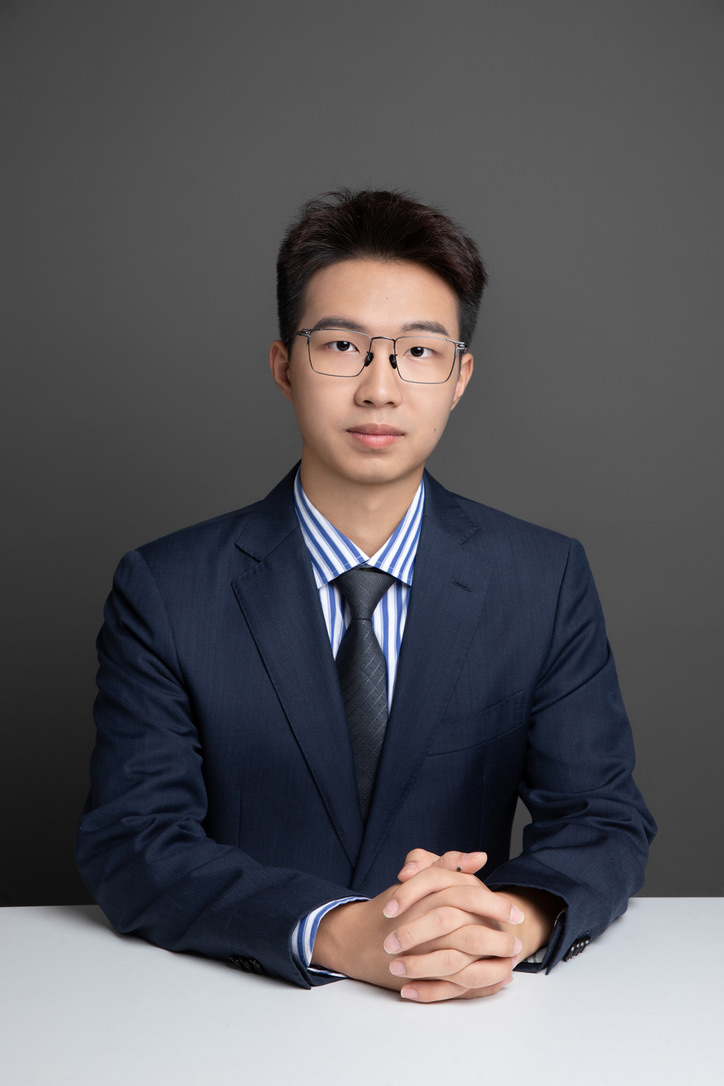
\includegraphics[width=2.55cm,height=3.25cm,keepaspectratio]{../assets/personal-professional-photo.jpeg}%
  }{%
    \fbox{\parbox[c][3.25cm][c]{2.55cm}{\centering \small 证件照}}%
  }%
}

\begin{document}

\noindent
\begin{minipage}[t]{0.79\textwidth}
{\LARGE \bfseries 周飞宇}\par
\vspace{2pt}
{\normalsize AI算法工程师｜Transformer、时序建模、Ray 分布式训练、机器人感知与 AI Agent / MCP 工具链}\par
\vspace{3pt}
邮箱：\href{mailto:feiyu.2002@outlook.com}{feiyu.2002@outlook.com}\quad
电话：+86 17326054065\par
现居：杭州，中国\quad
GitHub：\href{https://github.com/fatfishzhou}{github.com/fatfishzhou}\par
主页：\href{https://fatfishzhou.github.io}{fatfishzhou.github.io}\par
\end{minipage}
\hfill
\begin{minipage}[t]{0.17\textwidth}
\raggedleft
\vspace{0pt}
\ResumePhoto
\end{minipage}\par

\CVSection{职业概述}
\begin{itemize}
  \item 巴斯大学工程与设计人工智能硕士，当前主线聚焦 Transformer 与时序建模、Ray 分布式实验组织、模型训练流程与结果分析，目标方向为深度学习算法、训练基础设施与算法工程研发。
  \item 能够完成从数据处理、训练流程搭建、实验设计到结果验证与研究输出的完整研发闭环；同时具备 ROS2、点云链路、传感器接入与系统联调经验，可支撑算法与真实系统之间的落地连接。
  \item 已公开发表 2 篇期刊论文，其中第一作者 1 篇；另有 3 篇稿件在审或返修中、1 篇会议投稿；同时持续探索 AI Agent / MCP 工具链在研发提效中的工程化接入方式。
\end{itemize}

\CVSection{核心能力}
\textbf{算法与建模：}Python，NumPy，pandas，scikit-learn，PyTorch，PyTorch Lightning，Transformer，自注意力机制，时序建模，多变量信号分析，异常检测，实验设计，结果分析。\par
\vspace{2pt}
\textbf{训练基础设施与实验编排：}Ray，Ray Train，Ray Tune，并行实验管理，训练任务调度，参数搜索，实验配置组织，可复现性管理，模型训练闭环搭建。\par
\vspace{2pt}
\textbf{机器人感知与系统实践：}ROS2，Linux，四足机器人平台集成，Livox MID360，点云链路调试，激光惯性里程计方案分析，\texttt{grid\_map}，ESDF 建模思路，环境建模与系统联调。\par
\vspace{2pt}
\textbf{工程部署与研发工具链：}Docker，服务器与虚拟机环境，\texttt{vLLM} 本地推理部署，LLM API 接入与调试，Git，Rhino，3D 打印，Codex，Claude Code，MCP 系统实践，多智能体协作辅助研发。\par

\CVSection{代表项目经历}

\EntryHeader{风致结构健康监测与数字孪生建模}{2025.02 -- 2025.10}{University of Bath}{英国}
\begin{itemize}
  \item 构建基于 Transformer 的编码器-解码器模型，用于风致响应建模与数字孪生场景下的多模态时序预测，重点围绕序列建模、模型表达能力与实验设计展开。
  \item 独立完成数据预处理、训练流程搭建、实验设计、结果分析与论文撰写，形成从问题定义到研究输出的完整模型研发闭环。
  \item 使用 Ray Train / Tune 组织训练任务、并行实验与参数搜索，提升实验效率、结果对比能力与训练流程的可管理性。
  \item 相关成果以第一作者投稿至 \emph{Computers \& Structures}，当前已完成 minor revision。
\end{itemize}

\vspace{3pt}
\EntryHeaderSingle{训练流程组织与 Ray 并行实验编排实践}{贯穿多项目}
\Muted{个人技术主线 / 算法工程能力沉淀}\par
\begin{itemize}
  \item 将分散的训练脚本、实验配置与结果记录整理为可复用的实验流程，重点关注实验命名、参数管理、结果对比与研发可复现性。
  \item 使用 Ray 组织并行实验、训练调度与参数搜索，将模型开发从单次试验推进到可迭代、可比较、可复盘的工程化流程。
  \item 围绕 PyTorch 训练脚本、实验配置组织与结果归档方式，持续沉淀更适合算法工程和训练平台场景的研发基础设施能力。
\end{itemize}

\vspace{3pt}
\EntryHeaderSingle{四足机器人系统集成、感知建图与环境建模实践}{2025.12 -- 至今}
\Muted{个人项目 / 实验室方向探索}\par
\begin{itemize}
  \item 基于 Unitree Go2、云深处 Lite3 与 Livox MID360 完成传感器安装、支架设计、ROS2 工作区搭建、驱动接入与整机联调。
  \item 围绕 Faster-LIO、FAST-LIO2 等方案开展实验与参数分析，关注定位稳定性、建图质量与真实系统中的工程可用性。
  \item 结合 \texttt{grid\_map}、nvblox 与 ESDF 建模思路，探索通行性分析、实时环境建模与数字孪生展示相关流程。
  \item 使用 Rhino 与 3D 打印快速迭代传感器支架、防护件与结构件，缩短实验闭环周期并提升平台验证效率。
\end{itemize}

\vspace{3pt}
\EntryHeader{混凝土氯离子扩散系数预测}{2023.06 -- 2023.12}{浙江工业大学}{中国}
\begin{itemize}
  \item 使用 MLP 与 SVM 等方法预测混凝土氯离子扩散系数，验证归一化与虚拟样本生成对模型泛化性能的提升。
  \item 完成数据建模、实验比较、结果分析与论文撰写，成果以第一作者发表于 \emph{Sustainability}。
\end{itemize}

\vspace{3pt}
\EntryHeader{城市轨道交通全封闭风噪屏障气动性能研究}{2025.04 -- 2025.08}{浙江工业大学}{中国}
\begin{itemize}
  \item 参与全封闭风噪屏障在横风作用下的气动性能研究，建立分析与验证流程，输出可复现实验与仿真思路。
  \item 结合工程背景开展模型分析与性能评估，相关论文目前以第一作者身份处于在审状态。
\end{itemize}

\CVSection{研究成果}
\begin{itemize}
  \item \textbf{第一作者，已发表：}Fei-Yu Zhou, Ning-Jing Tao, Yu-Rong Zhang, Wei-Bin Yuan. ``Prediction of Chloride Diffusion Coefficient in Concrete Based on Machine Learning and Virtual Sample Algorithm.'' \emph{Sustainability}, 2023. DOI: \href{https://doi.org/10.3390/su152416896}{10.3390/su152416896}.
  \item \textbf{共同作者，已发表：}Marios Impraimakis, Feiyu Zhou, Andrew Plummer. ``An Information-Theoretic Method For Dynamic System Identification With Output-Only Damping Estimation.'' \emph{Journal of Dynamic Systems, Measurement, and Control}, 2026. DOI: \href{https://doi.org/10.1115/1.4071371}{10.1115/1.4071371}.
  \item \textbf{第一作者，返修中：}Feiyu Zhou, Marios Impraimakis (cor.). ``Transformer Large Language Model-Inspired Self-Attention Encoder-Decoder for Wind Structural Health Monitoring and Deep AI Learning Digital Twinning.'' \emph{Computers \& Structures}, minor revision.
  \item \textbf{第一作者，在审：}Feiyu Zhou, Nan-Ting Yu (cor.), Zheng Yu, Xinyu Zheng, Wei-Bin Yuan. ``Aerodynamic performance of fully enclosed wind-noise barriers for urban rail transit subjected to crosswind.'' Journal manuscript under review.
  \item \textbf{共同作者，在审/投稿：}另有 1 篇关于生成式 AI 与异常检测的期刊稿件在审，1 篇关于多模态异常检测的会议论文已投稿至 ARTISTE 2025。
\end{itemize}

\CVSection{教育经历}
\EntryHeader{巴斯大学（University of Bath）}{2024.09 -- 2026.01}{工程与设计人工智能 理学硕士（MSc）}{英国}
综合成绩：66.7/100（Merit）\par
\Muted{课程与研究重心：时序建模、深度学习、模型研发、实验设计与工程落地。}\par

\vspace{4pt}
\EntryHeader{浙江工业大学}{2020.09 -- 2024.06}{土木工程 学士}{中国}
\Muted{本科阶段形成结构工程与建模基础，后续研究与技能重心转向 AI、模型训练、机器人系统与算法研发。}\par

\CVSection{补充信息}
\begin{itemize}
  \item 工作方式偏工程导向与闭环导向，重视问题定义、模块职责、实验路径、结果证据与系统可维护性；面对新问题时，优先建立最小可运行闭环，再逐步补齐评估、文档与系统结构。
  \item 持续关注 AI Agent、多智能体协作与 MCP 工具链在研发提效中的实际接入方式，重点不在工具堆砌，而在可复用的任务拆解、上下文组织、代码辅助与问题推进流程。
\end{itemize}

\end{document}
